\documentclass[border=4pt]{standalone}
% Shared TikZ macros for the "Gaussian wave" amplitude diagrams.
% Each wave is drawn isolated inside a fixed-size cell, no axes, with an
% optional probability label placed just outside the bump.
\usepackage{tikz}
\usepackage{amssymb}
\usepackage{amsmath}
\usetikzlibrary{calc,arrows.meta}

\definecolor{waveblue}{HTML}{3A7CA5}
\definecolor{wavered}{HTML}{D1495B}

% \gaussiancell{x0}{y0}{sign}{height}{color}{basislabel}{highlight}{problabel}
% Draws one Gaussian bump centered at (x0,y0), cell width 2.4, height range +-1.1.
% sign: +1 upright, -1 flipped. height: 0..1 (fraction of max bump height 0.85).
% basislabel: basis-state ket, always placed BELOW the baseline; empty string = no label.
% highlight: 1 draws a thin colored box around the cell, 0 = none.
% problabel: probability value, always placed ABOVE the bump's peak; empty string = no label.
\newcommand{\gaussiancell}[8]{%
  \begin{scope}[shift={(#1,#2)}]
    \pgfmathsetmacro{\amp}{#4*0.85*#3}
    \pgfmathsetmacro{\wid}{0.30}
    \draw[black, line width=0.5pt] (-1.15,0) -- (1.15,0);
    \draw[#5, line width=1.3pt, samples=120, smooth, domain=-1.05:1.05]
      plot (\x, {\amp*exp(-(\x*\x)/(2*\wid*\wid))});
    \fill[#5, opacity=0.18, samples=120, domain=-1.05:1.05]
      plot (\x, {\amp*exp(-(\x*\x)/(2*\wid*\wid))}) -- (1.05,0) -- (-1.05,0) -- cycle;
    \ifnum#7=1
      \draw[wavered, line width=0.9pt] (-1.15,-0.65) rectangle (1.15,1.35);
    \fi
    \ifx&#6&
    \else
      \ifnum#3>0
        \node[anchor=north, font=\footnotesize] at (0, -0.35) {#6};
      \else
        \node[anchor=north, font=\footnotesize] at (0, -0.95) {#6};
      \fi
    \fi
    \ifx&#8&
    \else
      \node[anchor=south, font=\small] at (0, 0.95) {#8};
    \fi
  \end{scope}
}

% \wavegrid{rows}{cols}{dx}{dy}{cellfn} where cellfn takes (row,col,index)
% (grid layout handled inline per-figure instead, for full control over per-cell content)

% \meanline{x0}{y0}{width}{amp}{label}
% Draws a dotted horizontal line at height amp (in the same units as
% \gaussiancell's amplitude, i.e. peak height = 0.85 at amp=1) spanning
% `width` cells wide, centered at (x0,y0), with a small label to its right.
\newcommand{\meanline}[5]{%
  \begin{scope}[shift={(#1,#2)}]
    \pgfmathsetmacro{\amp}{#4*0.85}
    \draw[gray, line width=0.9pt, densely dotted] (-1.15,\amp) -- (#3-1.15,\amp);
    \ifx&#5&
    \else
      \node[gray, anchor=west, font=\footnotesize] at (#3-1.05,\amp) {#5};
    \fi
  \end{scope}
}

\begin{document}
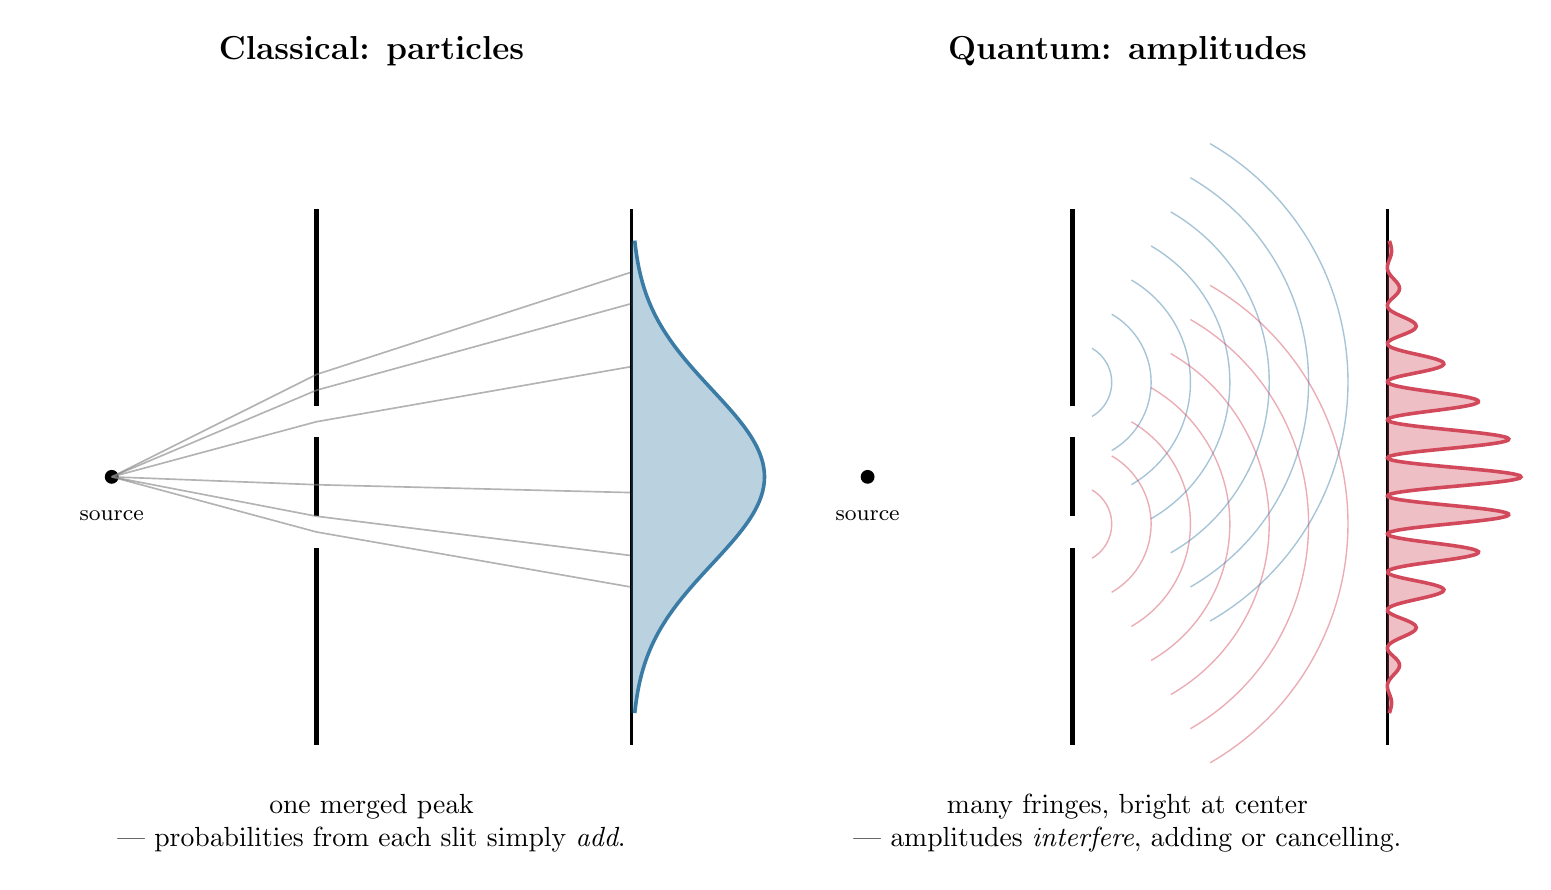
\begin{tikzpicture}
  % ---------- Left panel: classical (particles) ----------
  \node[font=\large\bfseries] at (0.1, 8.6) {Classical: particles};

  % source
  \fill[black] (-3.2,3.2) circle (2.5pt);
  \node[font=\footnotesize] at (-3.2,2.7) {source};

  % barrier with two slits
  \draw[black, line width=1.6pt] (-0.6,6.6) -- (-0.6,4.1);
  \draw[black, line width=1.6pt] (-0.6,3.7) -- (-0.6,2.7);
  \draw[black, line width=1.6pt] (-0.6,2.3) -- (-0.6,-0.2);

  % straight paths from source through each slit (particle trajectories)
  \foreach \y in {4.3,4.5,3.9} {
    \draw[gray, line width=0.6pt, opacity=0.6] (-3.2,3.2) -- (-0.6,\y) -- (3.4,{2*\y-3.2});
  }
  \foreach \y in {2.5,2.7,3.1} {
    \draw[gray, line width=0.6pt, opacity=0.6] (-3.2,3.2) -- (-0.6,\y) -- (3.4,{2*\y-3.2});
  }

  % screen
  \draw[black, line width=1.2pt] (3.4,-0.2) -- (3.4,6.6);

  % Classical intensity: incoherent sum of the two slits' single-slit
  % envelopes, I(y) = G(y-d/2) + G(y+d/2), each a non-negative Gaussian
  % envelope. In the far field d (slit separation) is tiny next to the
  % slit-to-screen distance, so the two envelopes sit almost on top of each
  % other and simply add -- one broadened peak at y=0, no zero-crossings.
  \pgfmathsetmacro{\dsep}{0.12}   % slit half-separation on the screen scale
  \pgfmathsetmacro{\senv}{1.1}    % envelope width
  \pgfmathsetmacro{\Iscale}{1.7}  % plot scale
  \draw[waveblue, line width=1.3pt, samples=150, smooth, domain=-3:3]
    plot ({3.4+\Iscale*(exp(-((\x-\dsep)*(\x-\dsep))/(2*\senv*\senv))+exp(-((\x+\dsep)*(\x+\dsep))/(2*\senv*\senv)))/2}, {3.2+\x});
  \fill[waveblue, opacity=0.35, samples=150, domain=-3:3]
    plot ({3.4+\Iscale*(exp(-((\x-\dsep)*(\x-\dsep))/(2*\senv*\senv))+exp(-((\x+\dsep)*(\x+\dsep))/(2*\senv*\senv)))/2}, {3.2+\x})
    -- (3.4,6.2) -- (3.4,0.2) -- cycle;

  \node[font=\normalsize, text width=8.5cm, align=center] at (0.1,-1.2)
    {one merged peak\\ --- probabilities from each slit simply \emph{add}.};

  % ---------- Right panel: quantum (wave interference) ----------
  \begin{scope}[shift={(9.6,0)}]
    \node[font=\large\bfseries] at (0.1, 8.6) {Quantum: amplitudes};

    \fill[black] (-3.2,3.2) circle (2.5pt);
    \node[font=\footnotesize] at (-3.2,2.7) {source};

    \draw[black, line width=1.6pt] (-0.6,6.6) -- (-0.6,4.1);
    \draw[black, line width=1.6pt] (-0.6,3.7) -- (-0.6,2.7);
    \draw[black, line width=1.6pt] (-0.6,2.3) -- (-0.6,-0.2);

    % expanding wavefronts from each slit (concentric arcs)
    \foreach \r in {0.5,1.0,1.5,2.0,2.5,3.0,3.5} {
      \draw[waveblue, line width=0.5pt, opacity=0.45] (-0.6,4.4) ++(-60:\r) arc (-60:60:\r);
      \draw[wavered, line width=0.5pt, opacity=0.45] (-0.6,2.6) ++(-60:\r) arc (-60:60:\r);
    }

    \draw[black, line width=1.2pt] (3.4,-0.2) -- (3.4,6.6);

    % Quantum intensity: coherent sum of the two slits' amplitudes,
    % I(y) = envelope(y) * cos^2(pi*d*y/lambda), the standard two-slit
    % interference pattern -- a bright fringe at y=0 (zero path difference,
    % constructive) flanked by symmetric side fringes, all under the same
    % single-slit envelope as the classical curve above.
    \pgfmathsetmacro{\kfringe}{6.5}  % fringe spatial frequency
    \draw[wavered, line width=1.3pt, samples=200, smooth, domain=-3:3]
      plot ({3.4+\Iscale*exp(-(\x*\x)/(2*\senv*\senv))*cos(\kfringe*\x*180/pi)*cos(\kfringe*\x*180/pi)}, {3.2+\x});
    \fill[wavered, opacity=0.35, samples=200, domain=-3:3]
      plot ({3.4+\Iscale*exp(-(\x*\x)/(2*\senv*\senv))*cos(\kfringe*\x*180/pi)*cos(\kfringe*\x*180/pi)}, {3.2+\x})
      -- (3.4,6.2) -- (3.4,0.2) -- cycle;

    \node[font=\normalsize, text width=8.5cm, align=center] at (0.1,-1.2)
      {many fringes, bright at center\\ --- amplitudes \emph{interfere}, adding or cancelling.};
  \end{scope}
\end{tikzpicture}
\end{document}
